\documentclass{article}
\usepackage{neurips_2025}

\usepackage[utf8]{inputenc}
\usepackage[T1]{fontenc}
\usepackage{hyperref}
\usepackage{url}
\usepackage{booktabs}
\usepackage{amsfonts}
\usepackage{nicefrac}
\usepackage{microtype}
\usepackage{xcolor}
\usepackage{amsmath}
\usepackage{graphicx}

\title{MedVQA-Router: Bridging Binary Classification and Open-Ended Captioning for Medical Visual Question Answering}

\author{
  Aisulu Tulyeujan \\
  Department of Computer Science \\
  University of Houston \\
  \texttt{aisulutulyeujan@gmail.com} \\
  \And
  Phuong Ho \\
  Department of Computer Science \\
  University of Houston \\
  \texttt{dho8@cougarnet.uh.edu} \\
  \And
  Micah Kuizon \\
  Department of Computer Science \\
  University of Houston \\
  \texttt{mkuizon@cougarnet.uh.edu} \\
  \And
  Sana Azhar \\
  Department of Computer Science \\
  University of Houston \\
  \texttt{sanaazhar59@gmail.com} \\
}

\begin{document}

\maketitle

% ============================================================
\begin{abstract}
Medical Visual Question Answering (Med-VQA) requires simultaneous understanding
of clinical images and natural-language questions. We address both the binary
(yes/no) and open-ended subsets of Med-VQA using the
\texttt{robailleo/medical-vision-llm-dataset}~\cite{robailleo2024}, which
contains 4,793 samples across X-ray, CT, MRI, and ultrasound modalities. Our
two-stage pipeline routes questions via a rule-based classifier, directing
binary questions to a multimodal fusion model (ResNet-18 + BioBERT) and
open-ended questions to GPT-5 Mini via the OpenAI API. For binary VQA we
compare text-only baselines (TF-IDF + LR/SVM), an image-only CNN (ResNet-18),
and fusion models. Our best binary classifier---ResNet-18 fused with fine-tuned
BioBERT---achieves \textbf{79.5\% accuracy} and \textbf{0.83 AUC-ROC},
outperforming single-modality baselines by over 7 percentage points. For the
open-ended branch, we evaluate four vision-language models and find that GPT-5
Mini achieves the highest BERTScore F1 (0.7528) and Recall (0.8021),
while InstructBLIP leads on ROUGE, demonstrating that GPT-5 Mini captures clinical
meaning more completely than smaller fine-tuned models.
\end{abstract}


% ============================================================
\section{Introduction}

Medical Visual Question Answering (VQA) has attracted significant research
interest as a tool for automated clinical decision support. A Med-VQA system
must jointly reason over a clinical image and a natural-language question to
produce a correct answer---either binary (``Is there a fracture?'') or
open-ended (``What abnormality is visible?''), requiring different modelling
strategies.

Medical datasets are limited in size due to the high cost of expert annotation
and privacy regulations. Clinical images exhibit significant visual diversity
across modalities, while questions use a highly specialized vocabulary. Standard
vision-language models pretrained on natural images often fail to capture subtle
pathological markers critical for accurate diagnosis.

We propose a two-stage pipeline that prioritizes task specialization: a routing
classifier separates binary from open-ended questions, directing each to a
dedicated model. For binary VQA, a multimodal fusion of ResNet-18 and BioBERT
achieves 79.5\% accuracy and 0.83 AUC-ROC, outperforming general-purpose models
like CLIP. For open-ended captioning, we evaluate a progression of four
vision-language models and find that GPT-5 Mini captures clinical meaning most
completely, achieving the highest BERTScore F1 (0.7528) and Recall
(0.8021).

% ============================================================
\section{Background}
\label{sec:background}

\textbf{Visual and Medical VQA.}
Since the VQA v2 dataset~\cite{goyal2017making}, VQA research has evolved from
monolithic architectures to complex attention-based mechanisms. In the medical
domain, datasets such as VQA-Med~\cite{lau2018dataset} and
SLAKE~\cite{liu2021slake} benchmark performance on radiology and pathology
images, where accuracy is safety-critical and linguistic bias is a known
challenge.

\textbf{Transfer Learning and Biomedical Language Models.}
Due to the scarcity of annotated medical images, transfer learning from
ImageNet-pretrained ResNet architectures~\cite{he2016resnet} is standard
practice. BERT~\cite{devlin2018bert} has spawned specialized variants such as
BioBERT~\cite{lee2020biobert}, pretrained on PubMed abstracts and PubMed
Central full texts, making it significantly better suited to clinical
terminology than general-domain models.

\textbf{Vision-Language Models.}
CLIP~\cite{radford2021clip} aligns images and text in a shared latent space
via dual encoders, while BLIP~\cite{li2022blip} enables flexible generation
through a multimodal encoder-decoder mixture. GPT-5 Mini extends this to
large-scale instruction-following captioning via the OpenAI API.


% ============================================================
\section{Data}
\label{sec:data}

\subsection{Dataset}
We use the \texttt{robailleo/medical-vision-llm-dataset}~\cite{robailleo2024}
from HuggingFace, a combined medical vision-language dataset comprising
\textbf{4,793 samples} drawn from two sources: ROCO (3,000 samples) and
VQA-RAD (1,793 samples). The official split yields \textbf{3,834 training} and
\textbf{959 validation} samples.

\textbf{Modality distribution:} X-ray dominates with 2,325 samples (48.5\%),
followed by CT (1,351; 28.2\%), unknown modality (812; 16.9\%), MRI (231;
4.8\%), ultrasound (70; 1.5\%), and microscopy/endoscopy (4; $<$0.1\%).
\textbf{Body-part distribution:} Unknown (2,856), chest (718), abdomen (468),
head (408), extremities (125), spine (119), and pelvis (99).

\begin{figure}[h]
    \centering
    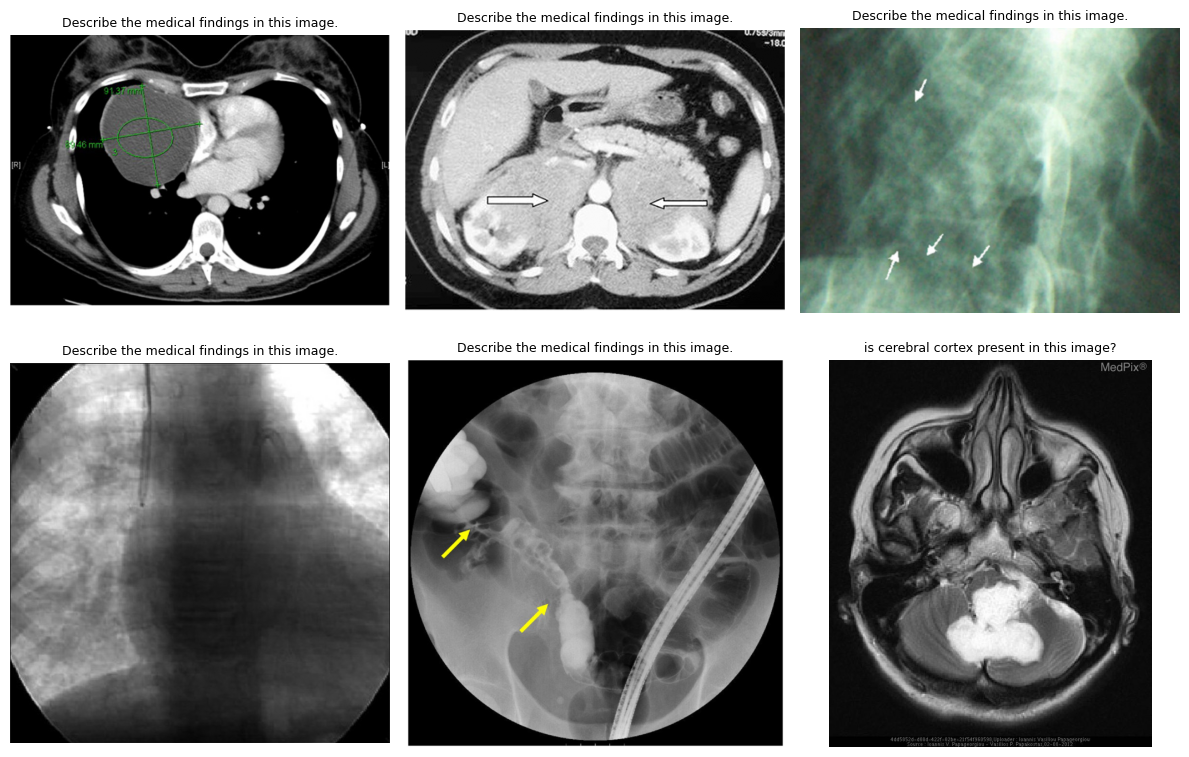
\includegraphics[width=0.75\textwidth]{figures/sample_images.png}
    \caption{Example medical images from the dataset. The dataset includes multiple medical imaging modalities such as X-ray, CT, MRI, and ultrasound.}
    \label{fig:sample-images}
\end{figure}

\subsection{Preprocessing and Split}
The preprocessing pipeline was designed to make the image and text data ready
for the model. Each image is resized to $224 \times 224$ pixels so that all
images have the same input size. Since some images are grayscale, every image is
converted to three-channel RGB format. After that, the image is converted into a
PyTorch tensor and normalized using ImageNet statistics with mean
$[0.485, 0.456, 0.406]$ and standard deviation $[0.229, 0.224, 0.225]$. This is
useful because the image encoder is based on pretrained CNN/ResNet models, which
expect images in this format.

For the text part, the question is kept as the input sentence for the text
encoder. Questions are tokenized with a maximum sequence length of 128 tokens.
Longer questions are truncated, and shorter questions are padded when needed.
This gives the model a fixed-size text input while still keeping the important
information from the question.

The dataset already provides official train and validation splits, so we did not
create a new random split for the main experiments. After filtering the dataset
to only binary yes/no examples, the binary training set contained 750 samples and
the binary validation set contained 190 samples. The class distribution stayed
balanced in both splits. In the training split, there were 379 no examples and
371 yes examples. In the validation split, there were 94 no examples and 96 yes
examples.

Because the predefined split was already balanced, we used it directly for
training and evaluation. We also checked the label percentages in each split:
the training split was about 50.53\% no and 49.47\% yes, while the validation
split was about 49.47\% no and 50.53\% yes. This showed that the official split
was reasonable for binary classification.

\begin{table}[h]
    \centering
    \caption{Binary label distribution after filtering to yes/no answers. Label 0 represents ``no'' and label 1 represents ``yes''.}
    \label{tab:binary-split-distribution}
    \begin{tabular}{lcc}
        \hline
        Split & Label 0 (No) & Label 1 (Yes) \\
        \hline
        Train & 379 & 371 \\
        Validation & 94 & 96 \\
        \hline
    \end{tabular}
\end{table}

% ============================================================
\section{Methods}
\label{sec:methods}

Our system has three components: (1) a routing classifier, (2) a binary VQA
pipeline, and (3) an open-ended captioning pipeline.

\begin{figure}[h]
  \centering
  
\includegraphics[width=0.92\linewidth]{figures/pipeline.png}
  \caption{End-to-end pipeline: the routing classifier directs inputs to the
           binary classification or open-ended captioning branch.}
  \label{fig:pipeline}
\end{figure}

\subsection{Routing Classifier}
\label{sec:routing}
A rule-based router in \texttt{src/utils.py} inspects each answer: ``yes'' or
``no'' answers are directed to binary classification; all others to open-ended
captioning. The routing is deterministic and error-free by construction,
operating on ground-truth answer labels across all 4,793 samples.

\subsection{Text-Only Baselines}
Questions are vectorized with TF-IDF (10,000 terms, \texttt{ngram\_range=(1,3)},
\texttt{sublinear\_tf=True}). We train Logistic Regression (L2,
\texttt{max\_iter=1000}) and SVM (linear kernel) on these features. TF-IDF +
SVM achieves 68.95\% accuracy and 0.75 AUC-ROC, confirming meaningful but
insufficient signal from text alone.

\subsection{Image-Only Baseline}
ResNet-18~\cite{he2016resnet} pretrained on ImageNet is fine-tuned with
\texttt{layer4} unfrozen and a new binary classification head, reusing
low-level ImageNet features while adapting high-level representations to the
medical domain.

\subsection{Multimodal Fusion Models}
\label{sec:fusion}

Our fusion model concatenates image and text features before a learned head:
\begin{itemize}
  \item \textbf{Image encoder}: ResNet-18 (\texttt{layer4} unfrozen), 512-dim
        after global average pooling.
  \item \textbf{Text encoder}: \\Frozen CLIP (512-dim)~\cite{radford2021clip} or
        BioBERT \texttt{dmis-lab/biobert-base-cased-v1.2}~\cite{lee2020biobert}
        (768-dim, mean-pooled last hidden state).
  \item \textbf{Fusion head}: LayerNorm on each stream $\rightarrow$
        concatenation $\rightarrow$ Linear(256)--ReLU--Dropout(0.5)--Linear(1).
\end{itemize}

The fused representation is:
\begin{equation}
  z_{\text{fused}} = \bigl[\,\text{LN}(z_{\text{img}}) \oplus \text{LN}(z_{\text{txt}})\,\bigr]
\end{equation}
\hspace{4.65cm} where $z_{\text{img}} \in \mathbb{R}^{512}$, $z_{\text{txt}} \in \mathbb{R}^{768}$.

BioBERT is chosen over CLIP because it is pretrained on PubMed abstracts and
PubMed Central texts, making it better suited to clinical terminology. We
additionally fine-tune BioBERT layers 10--11 at $5\times10^{-6}$ to adapt text
representations while avoiding catastrophic forgetting.

Models are trained with \texttt{BCEWithLogitsLoss} and AdamW with separate LR
groups: $10^{-4}$ (fusion head), $10^{-5}$ (ResNet \texttt{layer4}), $5\times
10^{-6}$ (BioBERT layers 10--11). Batch size 16, weight decay $10^{-4}$, up to
30 epochs, early stopping (patience 7), \texttt{ReduceLROnPlateau} (factor 0.5,
patience 3).

\subsection{Open-Ended Captioning Pipeline}
\label{sec:vlm}

We evaluate four vision-language models on the same 769-sample ROCO-derived
validation split, using BLIP variants as baselines and GPT-5 Mini as our
primary system.

As baselines, we evaluate three BLIP-family models: BLIP~\cite{li2022blip}
(224M parameters, also fine-tuned with frozen vision encoder on 3,084 samples),
BLIP-2~\cite{li2023blip2} (OPT-2.7B backbone, Q-Former bridging frozen ViT and
frozen LLM), and InstructBLIP~\cite{dai2023instructblip} (Vicuna-7B backbone,
instruction-conditioned Q-Former queries). These represent a progression in
architectural complexity and serve as reference points for evaluating GPT-5
Mini's capability.

\textbf{GPT-5 Mini}~\cite{openai2025} (\texttt{gpt-5-mini-2025-08-07}) is
queried via the OpenAI API, with each image base64-encoded and
submitted with the following system prompt:
\begin{quote}
\small\textit{``You are an expert radiologist interpreting medical images.
Provide concise, accurate, and specific medical descriptions using precise
clinical terminology. Focus only on what is visible in the image.''}
\end{quote}
Fine-tuning was withheld: the model weights are inaccessible for gradient
updates, fine-tuning via API raises reproducibility concerns, and zero-shot
performance is the relevant scenario when labeled medical data is scarce. 
Unlike the BLIP-family models, GPT-5 Mini generates structured
multi-sentence clinical reports, a consequence of the radiologist prompt that
produces the metric discrepancy discussed in
Section~\ref{sec:captioning-results}.

\textbf{Metrics.} We report BLEU-4, ROUGE-1, ROUGE-L, and
BERTScore~\cite{zhang2020bertscore} (P, R, F1 via DistilBERT). ROUGE measures
n-gram overlap and penalises verbosity. BERTScore uses contextual embeddings to
capture semantic similarity, correctly recognising that ``hepatic metastases''
and ``liver tumour'' are clinically equivalent despite zero lexical overlap.


% ============================================================
\section{Experiments}
\label{sec:experiments}

\subsection{Evaluation Metrics}
Binary VQA: accuracy, macro F1, and AUC-ROC on the 959-sample validation split.
Open-ended captioning: BLEU-4, ROUGE-L, and
BERTScore~\cite{zhang2020bertscore}.

\subsection{Binary VQA Results}

\begin{table}[h]
  \caption{Binary VQA model comparison on the validation set.}
  \label{tab:binary-results}
  \centering
  \begin{tabular}{lccc}
    \toprule
    Model & Accuracy & F1 & AUC-ROC \\
    \midrule
    TF-IDF + Logistic Regression             & 0.6684 & 0.6441 & 0.7073 \\
    TF-IDF + SVM                             & 0.6895 & 0.6704 & 0.7517 \\
    ResNet-18 (layer4 unfrozen)              & 0.7263 & 0.7500 & 0.7740 \\
    Fusion: ResNet-18 + CLIP                 & 0.7579 & 0.7723 & 0.8194 \\
    Fusion: ResNet-18 + BioBERT              & 0.7789 & 0.7835 & 0.8204 \\
    Fusion: ResNet-18 + BioBERT (fine-tuned) & \textbf{0.7947} & \textbf{0.8000} & \textbf{0.8281} \\
    \bottomrule
  \end{tabular}
\end{table}

Results show a clear progression from text-only baselines to multimodal fusion.
Moving from ResNet-18 alone (72.63\%) to CLIP fusion (+3.16 pp) confirms that
visual features alone are insufficient without textual grounding. Replacing CLIP
with BioBERT adds a further 2.1 pp, reflecting its stronger clinical vocabulary
alignment. We fine-tuned the last 2 layers of BioBERT on the dataset as suggested
from Prof. Lin, which improved accuracy from 77.9\% to 79.5\% (+1.6pp). Further 
improvement is limited by the dataset size (~750 training samples) — the model 
overfits heavily (train acc ~97\%) regardless of regularization strategy, 
suggesting more labeled data would be the real bottleneck to address.

\subsection{Open-Ended Captioning Results}
\label{sec:captioning-results}

\begin{table}[h]
  \caption{Open-ended captioning results on the validation set (769 samples).
           BLIP-2, InstructBLIP, and GPT-5 Mini are zero-shot. BERTScore uses
           DistilBERT embeddings. \textbf{Bold} = best per column.}
  \label{tab:captioning-results}
  \centering
  \small
  \begin{tabular}{lcccccc}
    \toprule
    Model & BLEU-4 & ROUGE-1 & ROUGE-L & BS-P & BS-R & BS-F1 \\
    \midrule
    BLIP             & 0.0000 & 0.0518 & 0.0427 & 0.6539 & 0.7019 & 0.6750 \\
    BLIP             & 0.0000 & 0.0953 & 0.0873 & 0.6812 & 0.7025 & 0.6905 \\
    BLIP-2           & 0.0039 & 0.1409 & 0.1251 & 0.7559 & 0.7304 & 0.7421 \\
    InstructBLIP     & 0.0058 & \textbf{0.1517} & \textbf{0.1345} & 0.7609 & 0.7353 & 0.7467 \\
    GPT-5 Mini       & \textbf{0.0088} & 0.1215 & 0.0943 & 0.7107 & \textbf{0.8021} & \textbf{0.7528} \\
    \bottomrule
  \end{tabular}
\end{table}
BERTScore F1 improves consistently across all five models (0.675 $\to$ 0.753),
reflecting genuine gains in semantic quality at each architectural step.
Fine-tuning BLIP's language decoder nearly doubles ROUGE-1 (0.052 to 0.095),
confirming that domain adaptation helps even at small scale. BLIP-2 surpasses
fine-tuned BLIP on all metrics despite no training on our data, showing that a
larger language backbone provides more value than task-specific adaptation with
limited samples.

GPT-5 Mini captures clinical meaning most completely, achieving the highest
BERTScore Recall (0.802) across all models, meaning it semantically covers the
reference findings more thoroughly than any fine-tuned alternative. Its lower
ROUGE score (0.122 vs.\ InstructBLIP's 0.152) is a product of output style
rather than quality: GPT-5 Mini generates structured clinical reports while
ROCO references are single-sentence labels, so ROUGE penalises length
asymmetry rather than inaccuracy. The lower Precision (0.711) similarly
reflects additional clinical detail beyond the reference. Taken together, these
results show that GPT-5 Mini is the strongest model in our evaluation when
assessed on semantic fidelity, and that ROUGE alone is insufficient for
evaluating models that generate richer text than their reference annotations.

\subsection{Qualitative Analysis}

For the binary branch, the BioBERT stream directed the classification head
toward image regions relevant to the specific organ in the query, with failure
cases concentrated in images with motion artifacts or fine-grained indicators
exceeding the $224\times224$ resolution. For the open-ended branch, the
following example illustrates the ROUGE--BERTScore discrepancy:

\begin{quote}
\small
\textbf{Reference:} \textit{Computed tomographic scan shows a metastatic liver
tumour (arrow).}\\[2pt]
\textbf{GPT-5 Mini:} \textit{Contrast-enhanced axial CT of the upper abdomen.
Numerous well-defined hypoattenuating nodules throughout the hepatic parenchyma
(several mm to $>$1\,cm), most consistent with multifocal hepatic metastases.
Peripheral/subcapsular lesion along the superior anterior hepatic surface
abutting the diaphragm (arrow). Impression: multifocal liver metastases;
subcapsular hepatic lesion.}
\end{quote}

Same diagnosis, near-zero lexical overlap. ROUGE scores this near zero;
BERTScore Recall of 0.802 correctly identifies high semantic coverage.

\subsection{Compute Resources}
Binary fusion experiments used NVIDIA T4 and A100 GPUs via Google Colab Pro,
requiring $\approx$45 minutes to converge over 30 epochs (batch size 16,
max sequence length 128). Open-ended experiments ran on an NVIDIA RTX 5070 Ti
(17.1\,GB VRAM) locally; BLIP fine-tuning completed in under 2 hours and each model took 30--45 minutes. GPT-5 Mini inference over 769 samples took
$\approx$2 hours via the OpenAI API.


% ============================================================
\section{Conclusion}
\label{sec:conclusion}

We presented MedVQA-Router, a two-stage pipeline for Medical VQA that routes
questions to a binary classification branch or an open-ended captioning branch.
Combining ResNet-18 with fine-tuned BioBERT achieves 79.5\% accuracy and 0.83
AUC-ROC, outperforming all single-modality baselines by over 7 pp. The
consistent advantage of BioBERT over CLIP confirms the value of domain-adapted
language models for medical text understanding. For the open-ended branch,
GPT-5 Mini achieves the highest BERTScore F1 (0.7528) and Recall (0.8021), 
while InstructBLIP leads on ROUGE, revealing that metric choice
critically shapes conclusions in medical captioning research. Future work
includes cross-attention fusion for finer-grained image-text interaction,
end-to-end multi-task routing, and evaluation on larger benchmarks such as
VQA-RAD and SLAKE~\cite{liu2021slake}.


% ============================================================
\begin{ack}
This project was completed as part of the COSC 4368 Fundamentals of Artificial
Intelligence course at the University of Houston. We thank Professor Sen Lin
and the course teaching assistants for their guidance throughout the semester.
\end{ack}


% ============================================================
\newpage
\bibliographystyle{plain}
\bibliography{references}


% ============================================================
\appendix

\end{document}